\documentclass{My_CV_Class}
\geometry{a4paper, total={170mm,257mm},left=20mm,top=20mm,}
\begin{document} 
\name{Naveen Kumar S}
\hspace{-6mm}
\line(1,0){450}
\begin{flushleft}
	\hspace{-1mm}
	6/20,Meal Eachavari,\\
	Ladduvadi Post,\\
	Namakkal-637002,\\
	Tamil Nadu.\\
	naveenkumarsingannan@gmail.com\\
	(+91)-9524821358
	\begin{picture}(0,0)
	\put(305,-3){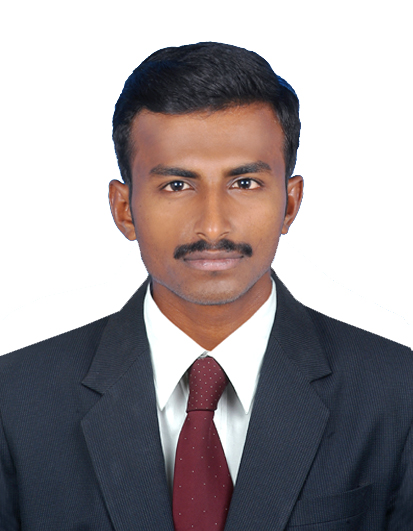
\includegraphics[width=20mm]{photo.jpg}}
	\end{picture}
\end{flushleft}
\vspace{5mm}
\section{Objective}
\hspace{6mm} Interested to work in inspiring, innovative workspace 
where I can learn new technology and realize my potential, 
which I can effectively contribute to the development of the organization
\section{Education}
\begin{tabular}{|c|c|c|c|c|}
	\hline
	Course & Institute & Board/University & Passing Year &  Percentage\\\hline
	B.E(EIE) & M.Kumarasamy College of   Engineering & Anna university & 2017 & 7.3\textsuperscript{*}\\\hline
	HSC & SKV Matriculation Higher Secondary School & State Board & 2013 & 73 \\\hline
	SSLC & SKV Matriculation Higher Secondary School & Matriculation & 2011 & 81.2 \\\hline
\end{tabular}
\begin{flushright}
	*upto 7th semester
\end{flushright}
\section{Project}
\begin{enumerate}
	\item TEMPERATURE TOLLERENCE CHECKING SYSYTEM
	\item SMART TRAFFIC SIGNS
	\item INTEGELLENT COLOUR IDENTIFIER
	\item SMART ENERGY METER
	\item LOCATION BASED SPEED GOVERNING DEVICE
	\item SMART HELMET
\end{enumerate}
\section{Training and Inernship}
\begin{itemize}
	\item Hands on training in Matlab
	\item PCB designing and fabrication
	\item Certified course in Hardware and networking
	\item Certified course in DCS
\end{itemize}
\section{Research and Publications}
\begin{enumerate}
	\item Presented a paper on the topic "STEERING OF SELF DIRECTED ROBOT"
\end{enumerate}
\section{Technical Skills}
\begin{itemize}
	\item Embedded c 
	\item embedded system designing using ATMega 328 microcontroller
	\item PCB designing and fabrication 
\end{itemize}
\newpage
\section{Software Skill Sets}
\begin{enumerate}
	\item Programming Languages : Embedded C, Python, Ladder Logics
	\item Operating System      : Windows, Debian Linux(Beginner)
\end{enumerate}
\section{Soft Skills}
\begin{itemize}
	\item Problem solving
	\item Adaptability
	\item Collaboration
\end{itemize}
\section{Extra-Curriclar Activities}
\begin{enumerate}
	\item Active participante in March Past event conducted in our college
	\item Active member of Citizen Consumer Club
	\item Act as a Join secretary of National Service Scheme during 2013-2015
\end{enumerate}
\section{Co-Curriclar Activities}
\begin{itemize}
	\item Won Second Prize for project in National Level Technical Symposium held in Sona College of Technology, Salem on 24th March 2016
	\item Won college level Second Prize in Project Expo 2015
	\item Conducted basic Hands on training on DCS, PLC Programming, SCDA in our college
\end{itemize}
\section{Personal Details}
Father's Name: S.SINGANNAN \\
Mother's Name: S.THANGAMMAL\\
Sex:		   MALE\\
Date of Birth: 23\textsuperscript{rd} JANUARY 1996\\
Nationality:   INDIAN\\
Marital Status:SINGLE
\section{Reference}
Dr.J.UMA\\
Head - Department of Electronics and Instrumentation Engineering\\
M.Kumarasamy College of Engineering\\
Ph:04324 - 270755 / 272155\\
Email : hodeie@mkce.ac.in
\end{document}
